\documentclass[border=10pt]{standalone}
\usepackage{tikz}\usepackage{amsmath}\usetikzlibrary{arrows.meta,decorations.markings}
\begin{document}
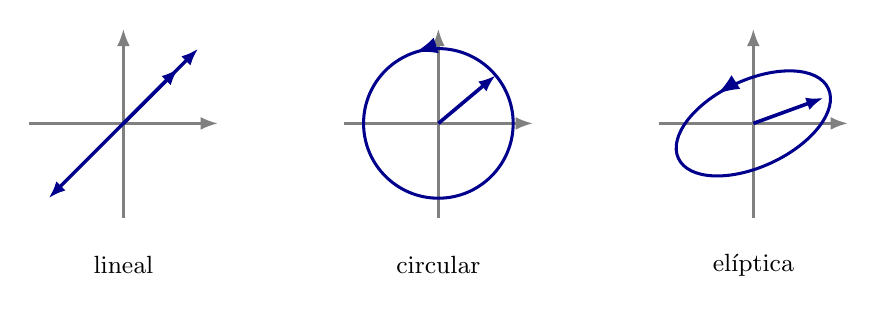
\begin{tikzpicture}[line width=0.9pt,>={Latex[length=2.2mm]}]
  % lineal
  \draw[->,gray] (-1.2,0)--(1.2,0); \draw[->,gray] (0,-1.2)--(0,1.2);
  \draw[<->,blue!55!black,line width=1.2pt] (-0.95,-0.95)--(0.95,0.95);
  \draw[->,blue!55!black,line width=1.3pt] (0,0)--(0.7,0.7);
  \node at (0,-1.8){\small lineal};
  % circular
  \begin{scope}[xshift=4cm]
    \draw[->,gray] (-1.2,0)--(1.2,0); \draw[->,gray] (0,-1.2)--(0,1.2);
    \draw[blue!55!black,line width=1.1pt,decoration={markings,mark=at position 0.3 with {\arrow{Latex}}},postaction={decorate}] (0,0) circle(0.95);
    \draw[->,blue!55!black,line width=1.3pt] (0,0)--(40:0.95);
    \node at (0,-1.8){\small circular};
  \end{scope}
  % eliptica
  \begin{scope}[xshift=8cm]
    \draw[->,gray] (-1.2,0)--(1.2,0); \draw[->,gray] (0,-1.2)--(0,1.2);
    \draw[blue!55!black,line width=1.1pt,rotate=25,decoration={markings,mark=at position 0.3 with {\arrow{Latex}}},postaction={decorate}] (0,0) ellipse (1.05 and 0.55);
    \draw[->,blue!55!black,line width=1.3pt] (0,0)--(20:0.95);
    \node at (0,-1.8){\small elíptica};
  \end{scope}
\end{tikzpicture}
\end{document}
